\part{Projektmanagement}

\chapter{Vorgehensmodell}


\chapter{Rollen und Verantwortlichkeiten}


\chapter{Risiken}\label{sec:risiken}


\chapter{Entwicklungsumgebung}


\section{Projektmanagement}


\chapter{Qualitätsmanagement}

\section{Reviews}

Um die Qualität der umgesetzten Tasks zu erhöhen und sicherzustellen wurde ein Review-Prozess eingesetzt. Jeder Task darf erst abgeschlossen werden, wenn ein anderes Teammitglied das Resultat grob angeschaut und für gut befunden hat. Um diesen Prozess einzuhalten wurde ein eigener Jira-Workflow verwendet.

\begin{figure}
\centering
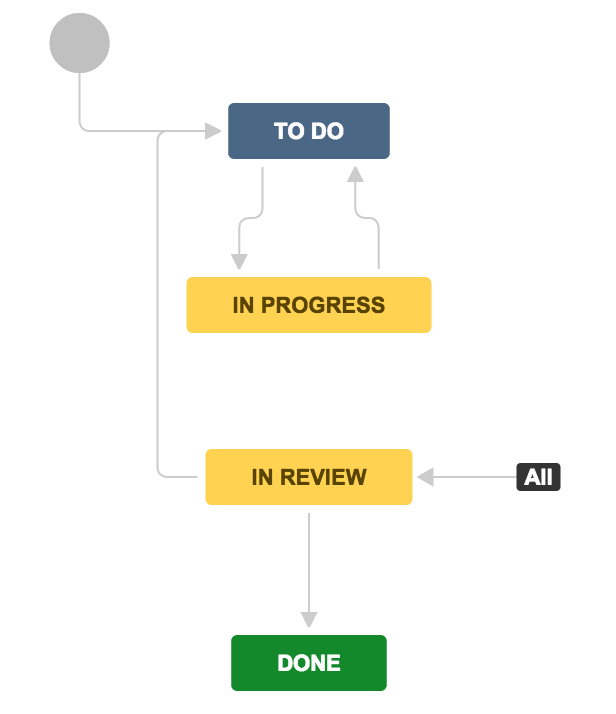
\includegraphics[width=0.7\linewidth]{content/projektmanagement/fig/jira-workflow}
\caption{Jira Review-Workflow}
\label{fig:jira-workflow}
\end{figure}

Der in \cref{fig:jira-workflow} dargestellte Prozess stellt sicher, dass alle Tasks erst in den Review Status versetzt werden müssen. Von diesem Status aus kann der Task entweder durch den Reviewer geschlossen oder zurück in den Status ''To Do'' versetzt werden, wobei bei letzterem der Tasks automatisch dem ursprünglichen Teammitglied zugewiesen wird.



\section{Tests}



\section{Coding-Richtlinien}


\subimport{sprints/}{sprints.tex}


